\chapter{Implementacja systemu}
	Ostateczna forma projektu przedstawiona została przy pomocy diagramów UML, wygenerowanych autorskim skryptem na podstawie kodu źródłowego gotowego programu.

\section{Warstwa rdzeniowa}
	W warstwie rdzeniowej ujęte zostały najczęściej używane struktury z pakietu Direct3D 11. Wrappery takich obiektów zostały oznaczone prefixem D3D. Pozostałe klasy posiadają nazwę bez przedrostków.

\subsection{Core}
	Klasa będąca podstawą funkcjonowania całego modułu. 
	Odpowiada za tworzenie oraz zarządzanie podstawowych zasobów używanych przez aplikacje oparte o Direct3D, takich jak Device, Context, RenderTarget(View), Swap Chain czy Framebuffer. Przy jego pomocy możliwy jest wybór trybu rysowania z listy reprezentowanej przez enum PrimitiveTopologies.
	Moduł zawiera także przez kompozycję odniesienie do obiektu klasy \textbf{Window}, która zawiera w sobie logikę odpowiedzialną za zarządzanie uchwytem do systemowego okna (i zasobami z tym związanymi) oraz odpowiedziami na zmianę jego stanu i rozmiaru.
	Inicjalizacja obu elementów odbywa się przez przekazanie w konstruktorze obiektu \textbf{WindowCreationParams}, zawierającego podstawowe informacje o tworzonym oknie.
	Diagram UML przedstawiony został na rys. \ref{UML_D3DCore}.
	
	
	\begin{figure}[ht!]
		\centering
		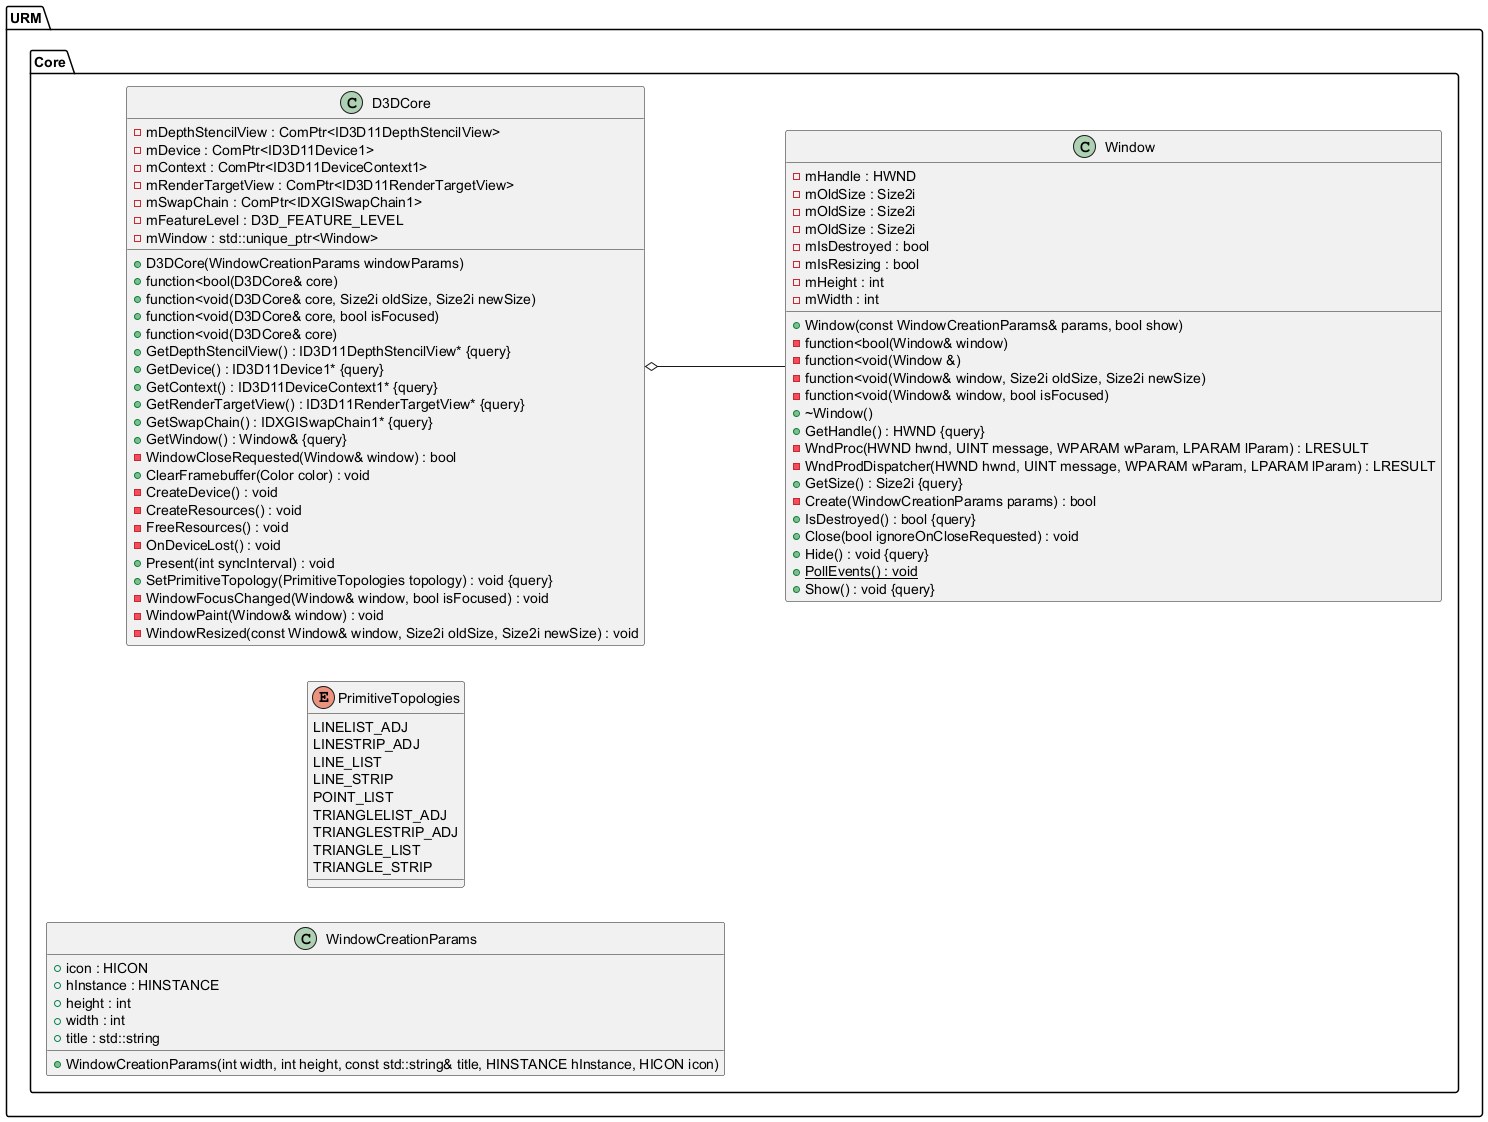
\includegraphics[width=\textwidth]{images/UML/core.png}
		\caption{Diagram UML przedstawiający kompozycję modułów D3DCore oraz Window wraz z zależnościami.}
		\label{UML_D3DCore}
	\end{figure}
	
	\vfill
	\clearpage
	
\subsection{Dziennik (Log)}
	Do prowadzenia dziennika \textit{(logu)} aktywności wykorzystana została otwartoźródłowa biblioteka \textbf{spdlog} na otwartej licencji MIT \cite{github:spdlog:spdlog}. Dodatkowo do modułu dołączona została statyczna klasa Logger opisana na rys. \ref{UML_Logger}. Udostępnia ona funkcje konfigurujące spdlog pod potrzeby projektu oraz metodę zwracającą referencję do dziennika zdarzeń krytycznych.
	

	\begin{figure}[h!]
		\centering
		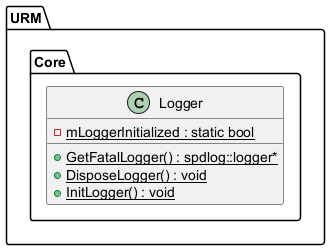
\includegraphics[width=\textwidth]{images/UML/logging.png}
		\caption{Schemat pomocniczej klasa statycznej dziennika.}
		\label{UML_Logger}
	\end{figure}
	
	\vfill
	\clearpage
	
\subsection{Metody pomocnicze}
	Sekcja zawierająca klasy i struktury pomocnicze wykorzystywane w ramach modułów projektu, przedstawione na rys. \ref{UML_Utils}.
	
	W ramach tego segmentu zaimplementowane zostały następujące klasy:
	\begin{itemize}
		\item \textbf{Size2i}: Prosta struktura opisująca rozmiar w przestrzeni 2D. Używana na przykład do określania wielkości okna.
		\item \textbf{TypeUtils}: Funkcje pomocnicze pobierania informacji o typach. Wykorzystywana między innymi do porównywania typów na podstawie wywołań generycznych.
		\item \textbf{StringUtils}: Odpowiedzialna za operacje tekstowe. Udostępnia funkcjonalność konwersji między zmiennymi tekstowymi jednobajtowymi \textit{(std::string)} oraz dwubajtowymi \textit{(std::wstring)}, a także pobierania nazwy folderu ze ścieżki do pliku.
		\item \textbf{FloatUtils}: Funkcjonalność ułatwiająca pracę z liczbami zmiennoprzecinkowymi. Dzięki metodom zawartym w tej klasie możliwe jest zbliżone porównywanie dwóch liczb typu float oraz określanie znaku tego typu liczb.
		\item \textbf{TimeUtils}: Wykorzystywana do testowania wydajności kodu. Pozwala na wywołanie dowolnej funkcji mierząc przy tym jej czas wykonania.
	\end{itemize}
	
	\begin{figure}[h!]
		\centering
		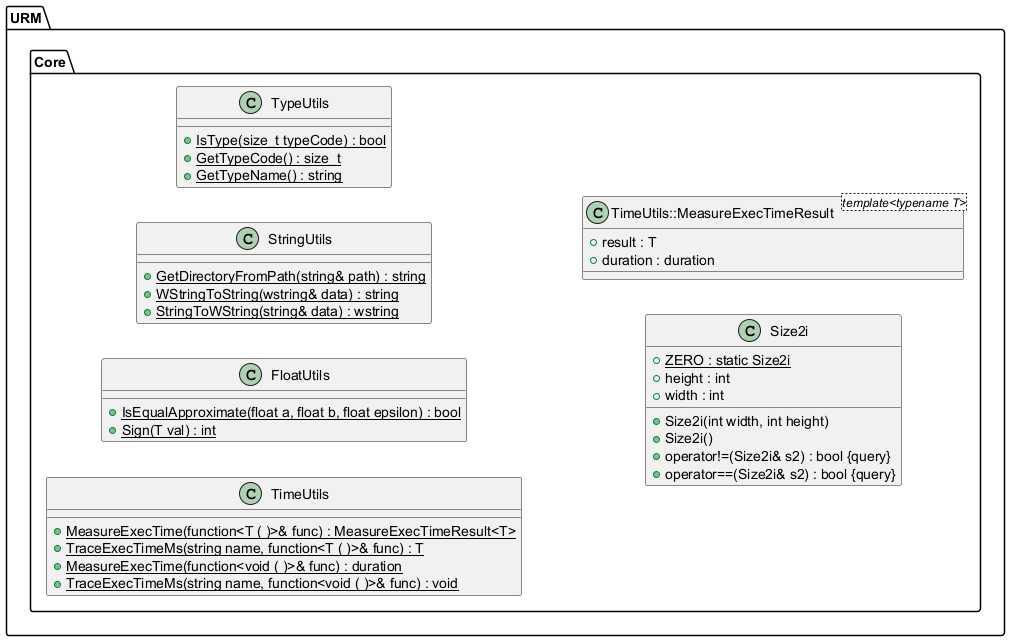
\includegraphics[width=\textwidth]{images/UML/utils.png}
		\caption{Schemat klas pomocniczych.}
		\label{UML_Utils}
	\end{figure}
	
	Do testów wydajności w trakcie oraz po zakończeniu prac nad modułem utworzona została także klasa \textbf{Stopwatch}, udostępniająca zaawansowaną funkcjonalność mierzenia czasu, a jej schemat został przedstawiony na rys. \ref{UML_Stopwatch}.
	
	\begin{figure}[h!]
		\centering
		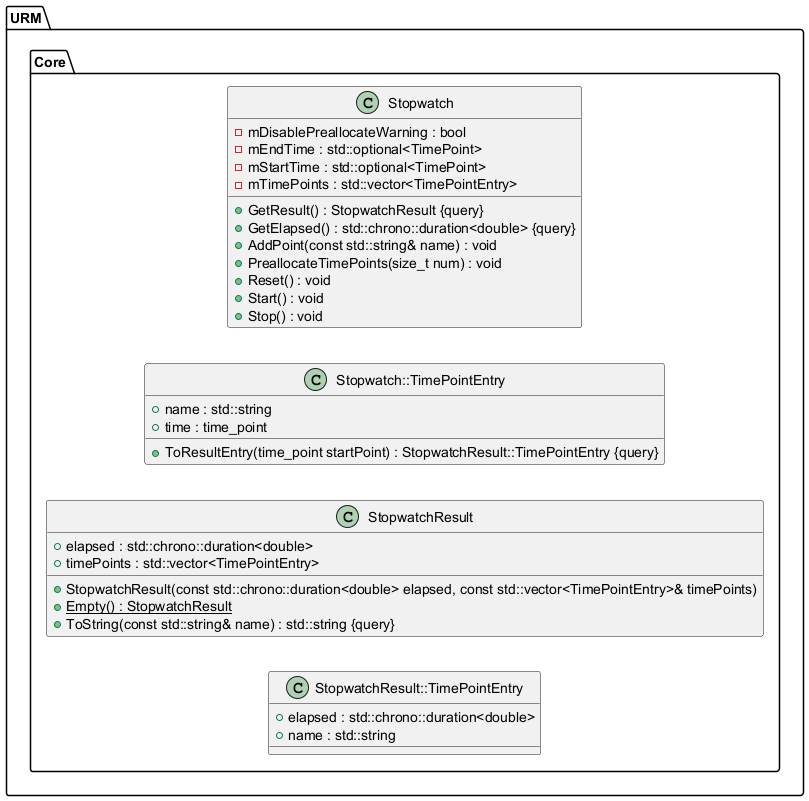
\includegraphics[width=\textwidth]{images/UML/stopwatch.png}
		\caption{Schemat klasy czasomierza.}
		\label{UML_Stopwatch}
	\end{figure}
	
\subsection{Baza D3D}
	Zbiór elementów będących warstwą abstrakcji nad niskopoziomowymi elementami pakietu Direct3D, wymaganych do jego użycia.
	\textbf{D3DViewport} odpowiedzialny jest za określanie wymiarów okna widoku (Viewport), jak i zakresu głębi rysowanego obrazu.
	Z kolei \textbf{D3DRasterizerState} pozwala na konfigurowanie parametrów procesu rasteryzacji, takich jak Culling Mode (definiowany przez enum CullModes) służący do pomijania wielokątów obróconych w złą stronę, tryb wypełnienia (przy pomocy enum FillModes), antyaliasingu, itp.
	Diagram przedstawiający strukturę opisywanych klas można zobaczyć na rys. \ref{UML_D3DUtils}
	
	\begin{figure}[h!]
		\centering
		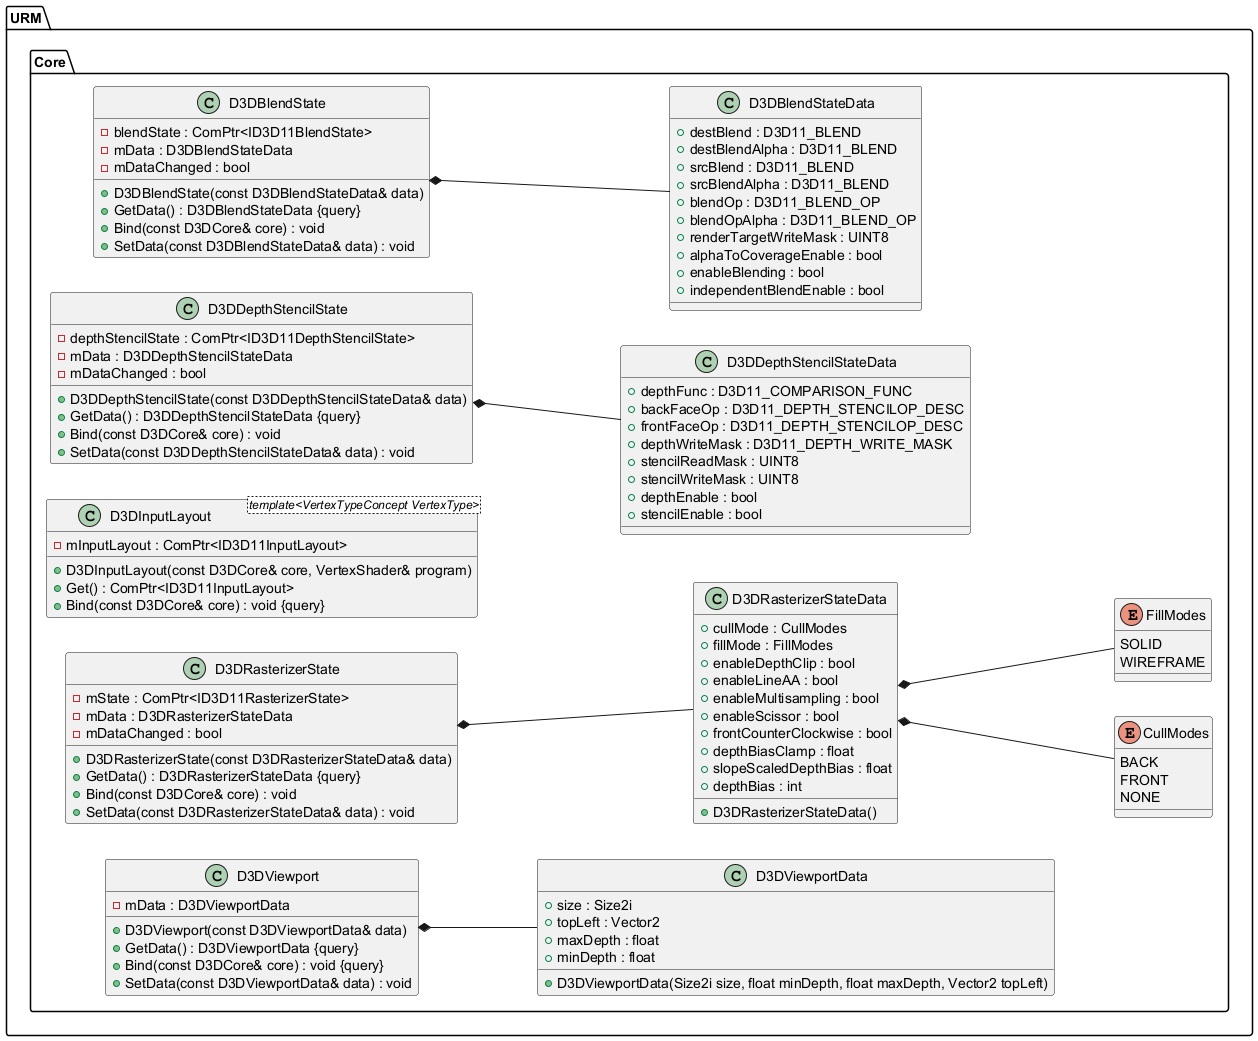
\includegraphics[width=\textwidth]{images/UML/d3dutils.png}
		\caption{Kompozycja wrapperów modułów bazowych D3D.}
		\label{UML_D3DUtils}
	\end{figure}
	
	\vfill
	\clearpage
	
\subsection{Bufory}
	Kolejnym elementem koniecznym do poprawnego korzystania z API D3D są bufory, używane jako środek przesyłu danych 
	Do ich łatwiejszej obsługi utworzona została klasa abstrakcyjna \textbf{ID3DBuffer}, której implementacje, \textbf{D3DVertexBuffer}, \textbf{D3DIndexBuffer} oraz \textbf{D3DConstantBuffer} stanowią rozwiązania do wykorzystania odpowiednio buforów wierzchołków, indeksów oraz stałych, a ich kompozycja została pokazana na rys. \ref{UML_Buffer}
	
		
	\begin{figure}[h!]
		\centering
		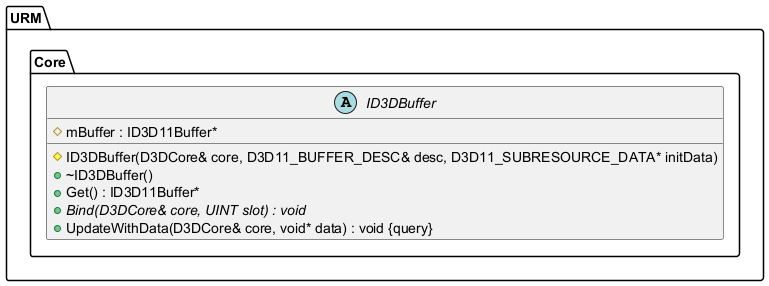
\includegraphics[width=\textwidth]{images/UML/buffer.png}
		\caption{Klasa ID3DBuffer oraz jej implementacje.}
		\label{UML_Buffer}
	\end{figure}
	
\subsection{Mesh i typy wierzchołków}
	Zbiór połączonych wielokątów wraz z opisującymi go metadanymi nazywany jest Mesh'em, którego schemat przedstawiony został na rys. \ref{UML_Mesh}.
	
	Zgodnie z założeniami projektu i ten element został zaprojektowany w modularnej formie. Wykorzystując szablon typów pozwala na pracę z różnymi typami wierzchołków. Kilka typów standardowych zostało zaimplementowanych w ramach modułu \textbf{StandardVertexTypes}, opisanego na diagramie \ref{UML_VertexTypes}.
	
	\begin{figure}[h!]
		\centering
		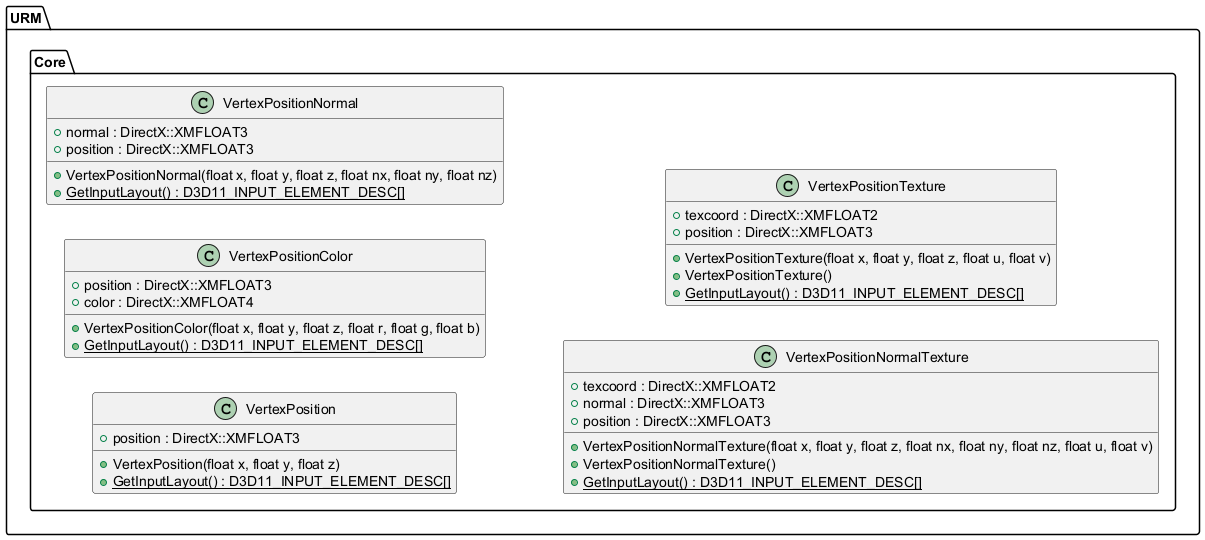
\includegraphics[width=\textwidth]{images/UML/vertextypes.png}
		\caption{Zaimplementowane standardowe typy wierzchołków.}
		\label{UML_VertexTypes}
	\end{figure}
	
	Do obsługi pozostałych typów wykorzystany został mechanizm \textit{concepts}, dodany w ramach standardu C++20 \cite{cpp20:concepts:2025}.
	Pozwala on na zdefiniowanie ograniczeń dla typu, co w opisywanym przypadku zostało wykorzystane do narzucenia konieczności implementacji statycznej metody \textit{std::vector<D3D11\_INPUT\_ELEMENT\_DESC> GetInputLayout()}, zwracającej wymaganą do poprawnej obsługi strukturę typu D3D11\_INPUT\_ELEMENT\_DESC.

	Dodatkowym elementem modularności jest obsługa modeli indeksowanych oraz nieindeksowanych, a także w razie potrzeby bezpośredni dostęp do wewnętrznych danych obiektu.
	
	Metadane przechowywane są jako lista wpisów typu \textbf{MaterialProperty}. Klasa ta obsługuje dane typów opisanych w enum \textbf{MaterialProperty::Types}, czyli typu buforowego, tekstowego \textit{(std::string)}, a także list liczb całkowitych \textit{(int)} i zmiennoprzecinkowych pojedynczej \textit{(float)} oraz podwójnej precyzji \textit{(double)}. Implementacja przechowuje te dane w postaci dynamicznie alokowanej i zwalnianej w destruktorze tablicy danych lub typu \textit{std::string}, a w celu zaoszczędzenia pamięci wykorzystany został moduł \textit{variant} ze standardu C++17 \cite{cpp17:variant:2025}. Przy pobieraniu danych następuje weryfikacja użycia poprawnego typu, który można sprawdzić używając metody \textit{GetType()}.
	
	\begin{figure}[h!]
		\centering
		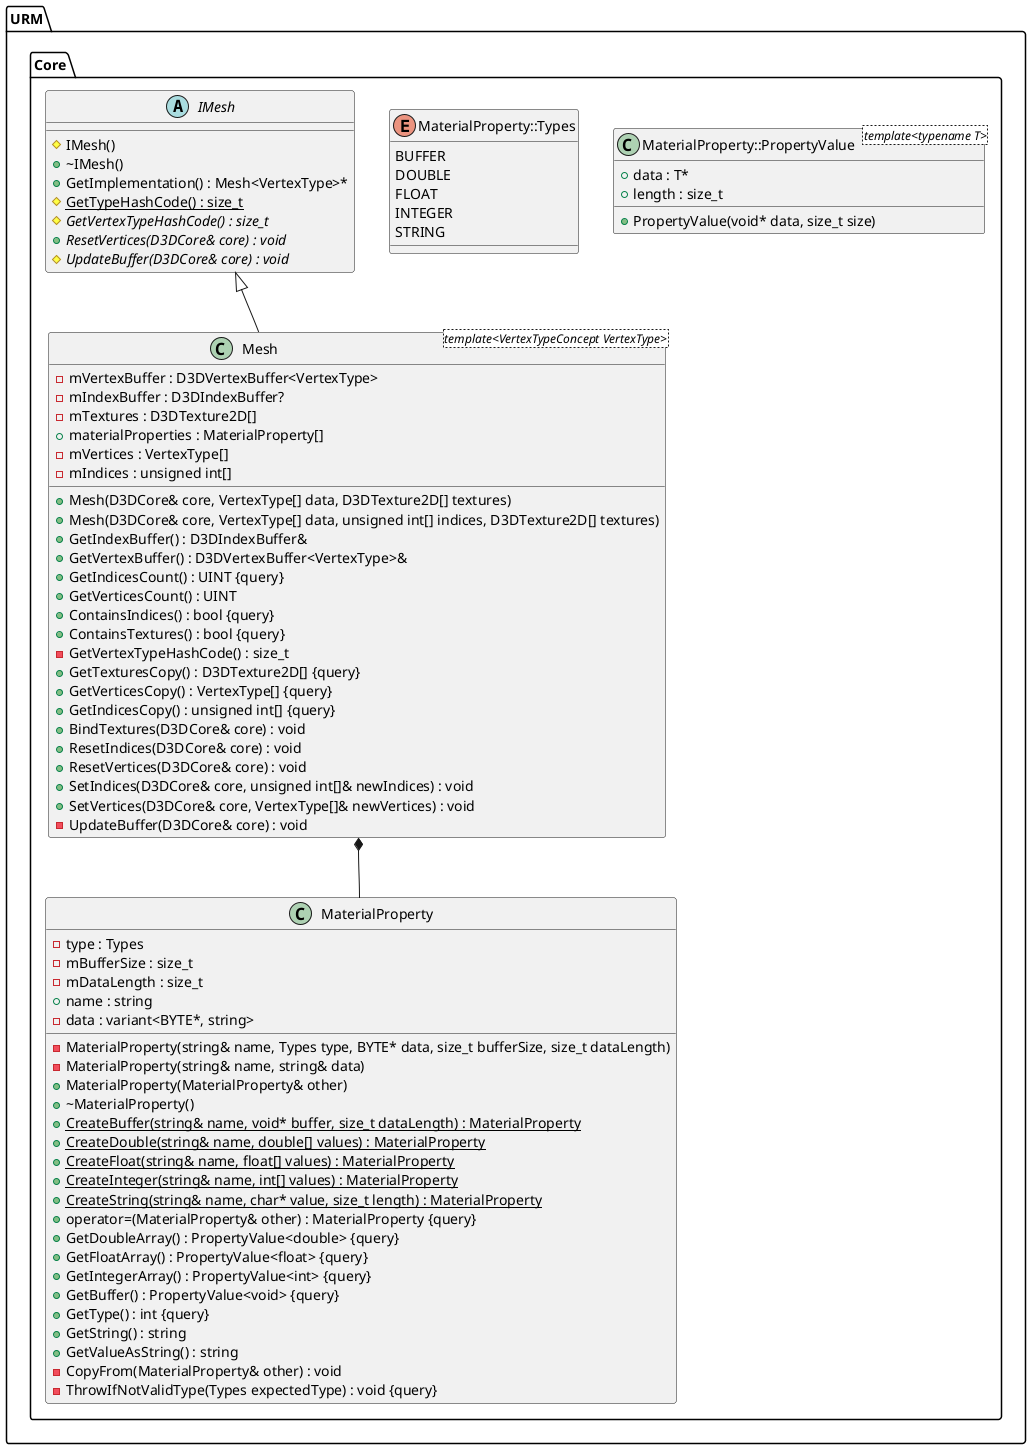
\includegraphics[width=\textwidth]{images/UML/mesh.png}
		\caption{Schemat klasy Mesh oraz klas wspierających.}
		\label{UML_Mesh}
	\end{figure}
	
		
	\vfill
	\clearpage
	
\subsection{Wczytywanie modeli}
	Funkcje pomocnicze ułatwiające wczytywanie modeli z pliku udostępnione zostały w ramach metod statycznych klasy \textbf{ModelLoader}. Metoda \textit{LoadFromFile()} jako argument otrzymuje ścieżkę do pliku modelu w obsługiwanym formacie, a następnie zwraca strukturę drzewową, której wierzchołkami są obiekty klasy \textbf{ModelLoaderNode}. Każdy wierzchołek zwracanego drzewa posiada macierz transformacji względem rodzica, listę mesh'y oraz wierzchołków przynależnych. Zachowywana zostaje oryginalna relacja transformacji między obiektami z wczytywanego pliku.
	Wraz z geometrią modelu wczytywane są także parametry metadanych do listy \textit{MaterialProperty} oraz przynależne do modelu tekstury. 
	
	Moduł obsługuje wszystkie formaty plików wspierane przez bibliotekę assimp, których pełna lista dostępna jest na stronie biblioteki \cite{github:assimp:FileFormats}. Szczególna uwaga została położona na wsparcie najczęściej spotykanych formatów, takich jak DAE, FBX, glTF / GLB, OBJ czy STL.
	
	Diagram opisywanych struktur został przedstawiony na rys. \ref{UML_ModelLoader}.
		
	\begin{figure}[h!]
		\centering
		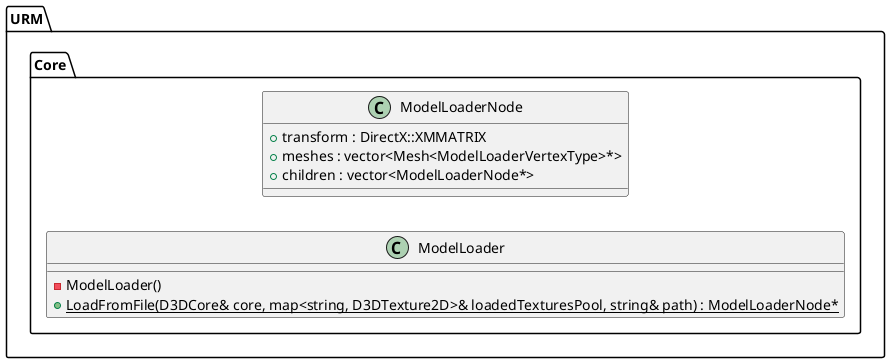
\includegraphics[width=\textwidth]{images/UML/modelloader.png}
		\caption{Schemat klasy statycznej ModelLoader wraz ze strukturą typu ModelLoaderNode.}
		\label{UML_ModelLoader}
	\end{figure}

\subsection{Tekstury}
	Kolejnym ważnym aspektem przy rysowaniu obiektów 3D są tekstury. Do reprezentacji ich dwuwymiarowych wersji powstała klasa \textbf{D3DTexture2D}, która przejmuje obowiązki wczytywania danych z pliku, utworzenia odpowiednich zasobów oraz zarządzania nimi. Istnieje także możliwość wczytania tekstury bezpośrednio z pamięci programu w formacie skompresowanym oraz nieskompresowanym.
	
	Do użycia z API D3D tekstury potrzebują także obiektu typu Sampler, który definiuje zachowanie próbkowania kolorów tekstury przy odczycie. Do ułatwienia tego zadania utworzona została klasa \textbf{D3DSampler}.
	
	Uproszczony schemat sekcji tekstur został opisany na rys. \ref{UML_Textures}.
	
	\begin{figure}[h!]
		\centering
		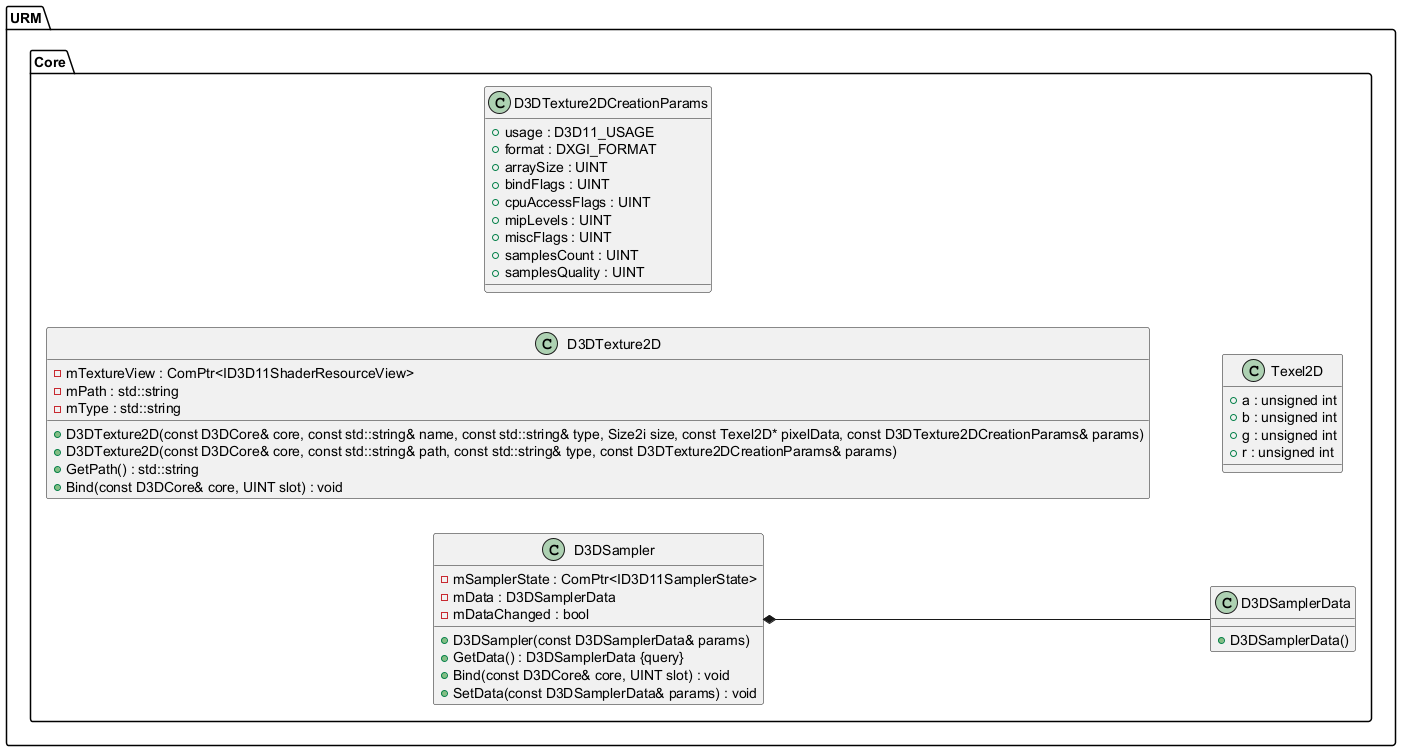
\includegraphics[width=\textwidth]{images/UML/texture.png}
		\caption{Schemat modułu tekstur.}
		\label{UML_Textures}
	\end{figure}
	
\subsection{Shader}
	W ramach modułu programy typy shader zostały zunifikowane do pojedynczej klasy, która reprezentuje poszczególne etapy procesu renderowania - \textbf{ShaderPipeline}. W aktualnej formie uwzględnia on etapy \textit{Vertex} oraz \textit{Pixel}, lecz dzięki modularnej budowanie możliwe jest uwzględnienie dodatkowych kroków, takich jak \textit{Geometry} czy \textit{Tesselation}.
	
	W ramach tego segmentu uwzględniony został także \textbf{D3DInputLayout}, służący jako warstwa abstrakcji nad układem wejściowym do shader'ów. Wykorzystuje on opisywany wcześniej koncept \textit{VertexTypeConcept} do automatycznego dopasowania w procesie rysowania modeli.
	
	Diagram UML segmentu został przedstawiony na rys. \ref{UML_ShaderPipeline}.
	
	\begin{figure}[h!]
		\centering
		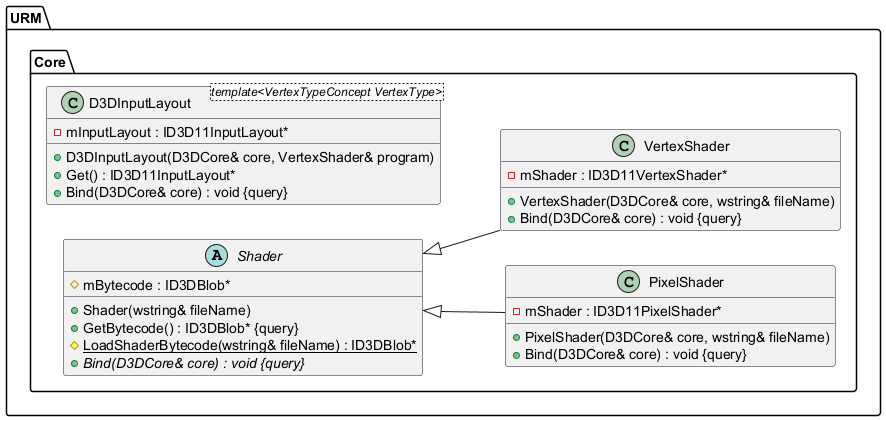
\includegraphics[width=\textwidth]{images/UML/shader.png}
		\caption{Schemat kompozycji klasy Shader oraz D3DInputLayout.}
		\label{UML_ShaderPipeline}
	\end{figure}